% ------------------------------------------------------------------ what I learned (1): course concepts
\begin{frame}{What I learned (1): course concepts at work}
    \label{sl:concepts}
    \scriptsize
    \renewcommand{\arraystretch}{1.08}
    \begin{tabular}{@{}c >{\raggedright\arraybackslash}p{0.345\linewidth} >{\raggedright\arraybackslash}p{0.465\linewidth} c@{}}
        \toprule
        & \textbf{Course concept} & \textbf{How TuneSight uses it} & \textbf{Slide}\\
        \midrule
        \tagS & Sampling, DFT/FFT, windowing, STFT & the ring frequencies (modes) of each strike, and how fast each fades & \pageref{sl:hearing}\\
        \tagS & LTI systems, impulse response, linear prediction, source--filter model & the tap is the source, the bowl the filter; LPC cross-checks the modes & \pageref{sl:hearing}\\
        \tagV & Thresholding (Otsu), morphology, contours & bowl silhouettes from a backlit frame & \pageref{sl:vision}\\
        \tagV & Colour spaces (HSV), intensity profiles & the water line from row saturation (edge step for clear water) & \pageref{sl:vision}\\
        \tagV & Camera geometry, fiducial markers & centimetres and millilitres from an ArUco marker & \pageref{sl:vision}\\
        \tagM & Regression, Bayesian inference, model evidence & learning the law online, and choosing its exponent & \pageref{sl:learning}\\
        \tagM & Multisensory integration, cue reliability, inverse effectiveness & weighted fusion of audio and striker motion, plus a ``none'' check & \pageref{sl:fusion}\\
        \bottomrule
    \end{tabular}
    \vspace{2mm}
    \begin{block}{What joining them taught me}
        \scriptsize
        One physical law ties the course topics together: audio \emph{labels} vision (fill $\to$ pitch), and fusion
        weighs each sense strike by strike. \hfill {\tiny\tagS{} sound \ \tagV{} images \ \tagM{} multimodal}
    \end{block}
\end{frame}

% ------------------------------------------------------------------ what I learned (2): lessons
\begin{frame}{What I learned (2): lessons beyond the formulas}
    \label{sl:lessons}
    \centering
    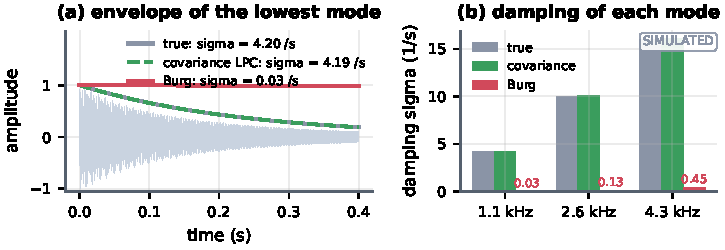
\includegraphics[width=0.76\linewidth]{images/figures/fig_burg.pdf}\\[-0.5mm]
    {\tiny Lesson 2 in one picture: on a decaying ring Burg's method finds almost no damping; the covariance method is exact.\par}
    \vspace{1.5mm}
    \begin{columns}[T]
    \column{0.5\textwidth}
        \scriptsize
        \begin{enumerate}
            \item \textbf{A law beats a dataset.} With the right physics, 5 taps give \EfiveFive~cents; a black box would need many labelled strikes.
            \item \textbf{Check a method's assumptions.} The textbook method (Burg \cite{burg1975maximum}) assumes a sound that does
                  not fade; a ringing bowl fades, so it got the fading 99\,\% wrong. A method without that assumption \cite{kumaresan1982estimating} is exact.
        \end{enumerate}
    \column{0.48\textwidth}
        \scriptsize
        \begin{enumerate}\setcounter{enumi}{2}
            \item \textbf{Fusion pays where a sense is weak:} at 0~dB, audio alone \EsixAudioZero\,\%, fused \EsixFusedZero\,\%.
            \item \textbf{Two clocks, one event:} align video to the audio onset; read the water \emph{before} the strike, when no hand hides it.
            \item \textbf{Simulate with ground truth first:} every module was tested against known answers before real data.
        \end{enumerate}
    \end{columns}
\end{frame}

% ------------------------------------------------------------------ reflections (a): surprises
\begin{frame}{Reflections (a): what surprised me}
    \label{sl:surprised}
    \begin{columns}[T]
    \column{0.39\textwidth}
        \centering
        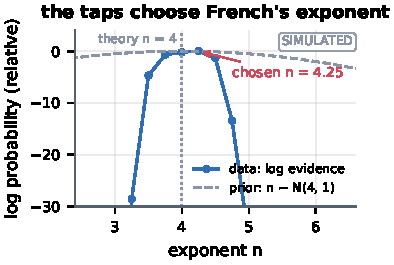
\includegraphics[width=0.96\linewidth]{images/figures/fig_evidence.pdf}
    \column{0.59\textwidth}
        \scriptsize
        \begin{itemize}
            \item \textbf{The data found the physics:} model evidence chose $n = \EthreeN$, French's exponent, with no tuning (left).
            \item \textbf{The textbook estimator failed:} Burg's method found almost no damping (slide \pageref{sl:lessons}).
            \item \textbf{Motion pointed at the wrong bowl:} the stick's body sweeps over the neighbour; only its tip is reliable.
            \item \textbf{``Identical'' is not identical:} a 3\,\% shape spread costs \EsevenDiffVision~cents; one tap brings it to \EsevenDiffTap.
        \end{itemize}
    \end{columns}
    \vspace{1mm}
    \centering
    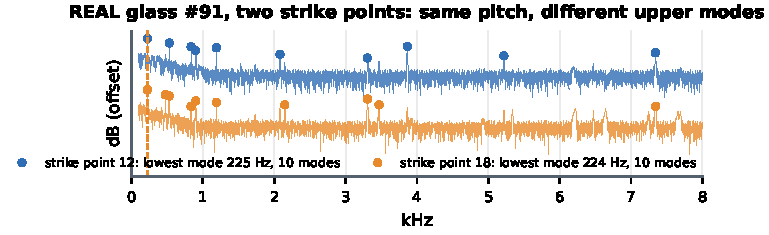
\includegraphics[width=0.80\linewidth]{images/figures/fig_strikepoint.pdf}\\[-0.5mm]
    {\tiny A real glass: the strike point changes the upper modes, not the lowest one (225 vs 224~Hz). One recording also has a 79~Hz line
    from the stand or room, 6~dB below the glass: searching from 60~Hz, it is taken as the pitch. A sensible band matters.\par}
\end{frame}

% ------------------------------------------------------------------ reflections (b): scope for improvement
\begin{frame}{Reflections (b): scope for improvement}
    \label{sl:improve}
    \centering
    \resizebox{\linewidth}{!}{%
    \begin{tikzpicture}[>={Stealth[length=2.5mm]}]
        \node[road=fusc] (r1) at (0, 0) {\textcolor{fusc}{\textbf{Next: real data}}\\[4pt]
            $\bullet$ Record a full session with real bowls and a musician\\[3pt]
            $\bullet$ Ruler check of the water line; real calibration and tuning results\\[3pt]
            $\bullet$ Mesh data for the size-scaling experiment (E2)};
        \node[road=camc] (r2) at (3.75, 0) {\textcolor{camc}{\textbf{Then: harder scenes}}\\[4pt]
            $\bullet$ Opaque porcelain bowls, as in a traditional jal tarang: a top-view or depth camera\\[3pt]
            $\bullet$ Two strikers and overlapping notes: multi-pitch analysis\\[3pt]
            $\bullet$ Reflections: a small learned water-line detector with the physics as its prior};
        \node[road=phyc] (r3) at (7.5, 0) {\textcolor{phyc!75!black}{\textbf{Later: beyond music}}\\[4pt]
            $\bullet$ Closed-loop tuning with a small pump\\[3pt]
            $\bullet$ A phone app: camera and mic in one device\\[3pt]
            $\bullet$ ``Tap and look'' level checks for rows of identical containers (bottles, tanks)};
        \foreach \x in {0, 3.75} \draw[->, thick, gray] (\x + 1.73, -1.0) -- (\x + 2.02, -1.0);
    \end{tikzpicture}}
    \vspace{2mm}
    \begin{alertblock}{Honest limitations today}
        \scriptsize
        Most results are simulated with known ground truth; the real audio is two ObjectFolder strikes of one glass.
        LPC damping degrades quickly with noise (1.4\,\% error at 40~dB, 54\,\% at 20~dB), and clear water needs the weaker edge cue.
    \end{alertblock}
\end{frame}

% ------------------------------------------------------------------ live demo and conclusion
\begin{frame}{Live demo and conclusion}
    \label{sl:demo}
    \begin{columns}[T]
    \column{0.54\textwidth}
        \centering
        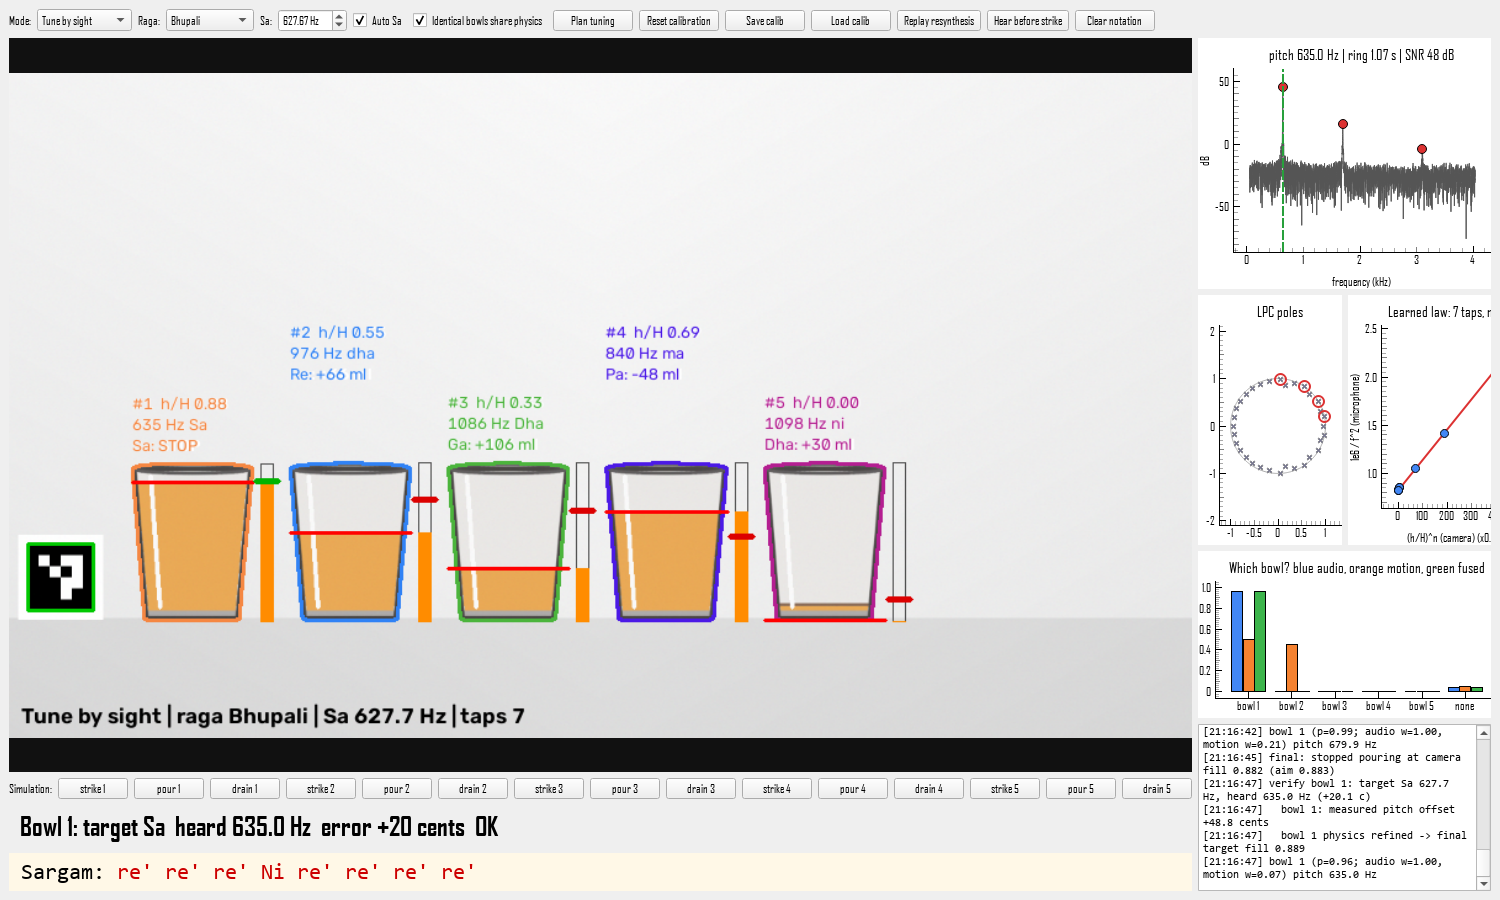
\includegraphics[width=\linewidth]{images/figures/app_screenshot.png}\par
        {\tiny Desktop app (webcam + mic, or \texttt{--sim}): water lines, targets, spectrum, LPC poles, learned law.\par}
        \vspace{2mm}
        \begin{minipage}[c]{0.52\linewidth}
            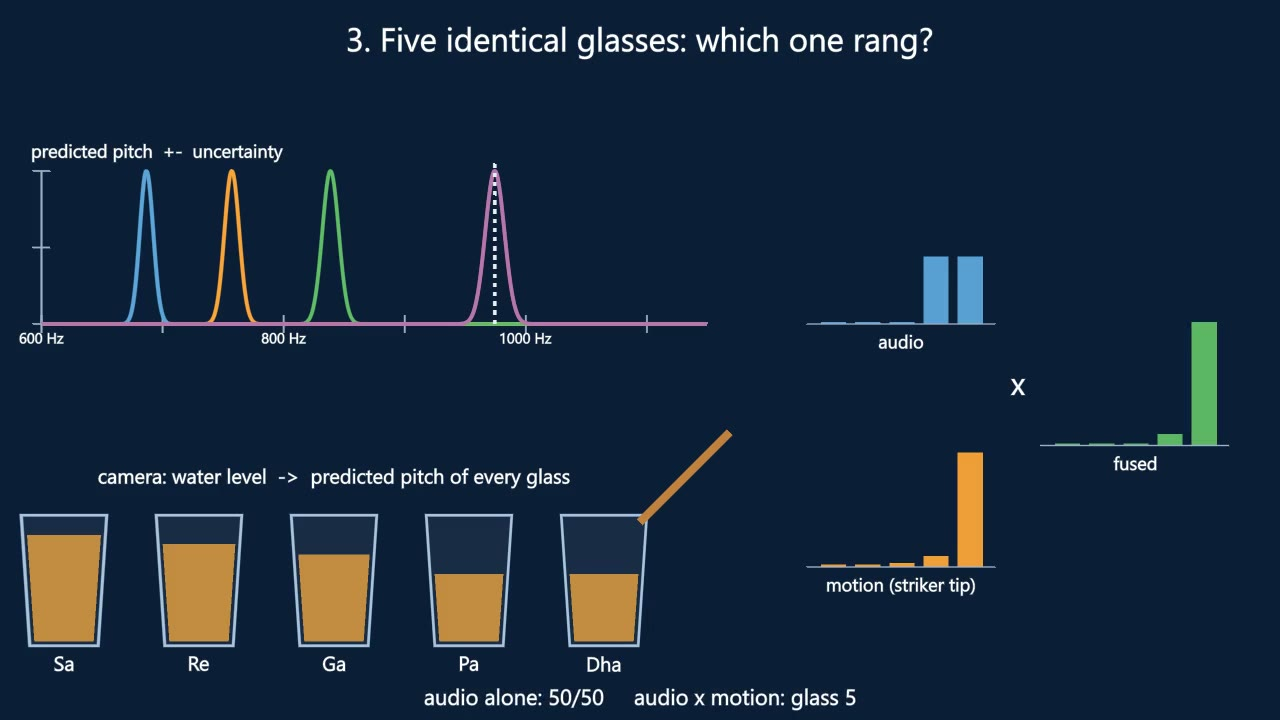
\includegraphics[width=\linewidth]{images/figures/anim_which.jpg}
        \end{minipage}\hfill
        \begin{minipage}[c]{0.45\linewidth}
            \raggedright\tiny
            Explainer page \texttt{web/index.html}: five ManimGL animations, the architecture diagram and five live in-browser demos.
        \end{minipage}
    \column{0.44\textwidth}
        \begin{exampleblock}{Conclusion}
            \scriptsize
            \begin{itemize}
                \item One physical law lets each modality predict the other.
                \item Fusion solves what neither sense can alone: identical bowls, noise, pitch ties.
                \item A few taps calibrate it; it then tunes a jal tarang by sight and writes the sargam.
            \end{itemize}
        \end{exampleblock}
        \begin{block}{Try it}
            \scriptsize
            \texttt{python app/app.py --sim}\\
            \texttt{python app/app.py} \hfill(webcam + mic)\\
            open \texttt{web/index.html}\\[2pt]
            \texttt{github.com/KUSHAGRA2606/TuneSight}
        \end{block}
    \end{columns}
\end{frame}
